\documentclass[12pt,preprint]{aastex}
\usepackage{amsmath}
\usepackage[]{graphicx, epstopdf}
\usepackage{indentfirst}
\usepackage{lscape}
\usepackage{afterpage}
\usepackage{rotating}
\let\captionbox\undefined
%\usepackage{caption}

%\captionsetup{width=6.3in,font=footnotesize}
\usepackage{wrapfig}
\usepackage{multicol}
\usepackage{textcomp}
\newcommand{\textapprox}{\raisebox{0.5ex}{\texttildelow}}

\usepackage{tabu}
\usepackage{multirow}

\usepackage{xcolor}
\usepackage{ulem}

\setlength{\textwidth}{6.5in}
\setlength{\hoffset}{0in}
\setlength{\oddsidemargin}{0in}
\setlength{\evensidemargin}{0in}

\setlength{\textheight}{9.in}
\setlength{\voffset}{0in}
\setlength{\topmargin}{0in}
\setlength{\headsep}{0.25in}
\setlength{\headheight}{0in}


%Some handy-dandy commands
%***Distance and Length***
\newcommand{\meters}{\mbox{m}}
\newcommand{\cm}{\mbox{cm}}
\newcommand{\km}{\mbox{km}}
\newcommand{\dpc}{d_{pc}}
\newcommand{\au}{\mbox{AU}}
\newcommand{\microns}{\mu\mbox{m}}
\newcommand{\rsun}{R_{\sun}}
\newcommand{\rjup}{R_J}
\newcommand{\rearth}{R_{\earth}}

%***Times***
\newcommand{\hours}{\mbox{ hrs}}
\newcommand{\seconds}{\mbox{ s}}
\newcommand{\years}{\mbox{ yrs}}

%**Mass**
\newcommand{\kg}{\mbox{kg}}
\newcommand{\msun}{M_{\sun}}
\newcommand{\mearth}{M_{\earth}}
\newcommand{\mjup}{M_J}






% Alter some LaTeX defaults for better treatment of figures:
    % See p.105 of "TeX Unbound" for suggested values.
    % See pp. 199-200 of Lamport's "LaTeX" book for details.
    %   General parameters, for ALL pages:
    \renewcommand{\topfraction}{0.9}    % max fraction of floats at top
    \renewcommand{\bottomfraction}{0.8} % max fraction of floats at bottom
    %   Parameters for TEXT pages (not float pages):
    \setcounter{topnumber}{2}
    \setcounter{bottomnumber}{2}
    \setcounter{totalnumber}{4}     % 2 may work better
    \setcounter{dbltopnumber}{2}    % for 2-column pages
    \renewcommand{\dbltopfraction}{0.9} % fit big float above 2-col. text
    \renewcommand{\textfraction}{0.07}  % allow minimal text w. figs
    %   Parameters for FLOAT pages (not text pages):
    \renewcommand{\floatpagefraction}{0.7}      % require fuller float pages
        % N.B.: floatpagefraction MUST be less than topfraction !!
    \renewcommand{\dblfloatpagefraction}{0.7}   % require fuller float pages

%%%%%%%%%%%%%%%%%%%%%%%%%%%%%%%%%%%%%%%%%%%%%%%%%%%%%%%%%%%%%%%%%%%%%%%%%%%%%%%%
%%
%% The following section outlines numerous optional output that
%% can be displayed in the front matter or as running meta-data.
%%
%% If you wish, you may supply running head information, although
%% this information may be modified by the editorial offices.
\shorttitle{Sample article}
\shortauthors{Schwarz et al.}
%%
%% You can add a light gray and diagonal water-mark to the first page 
%% with this command:
% \watermark{text}
%% where "text", e.g. DRAFT, is the text to appear.  If the text is 
%% long you can control the water-mark size with:
%  \setwatermarkfontsize{dimension}
%% where dimension is any recognized LaTeX dimension, e.g. pt, in, etc.
%%
%%%%%%%%%%%%%%%%%%%%%%%%%%%%%%%%%%%%%%%%%%%%%%%%%%%%%%%%%%%%%%%%%%%%%%%%%%%%%%%%

%% This is the end of the preamble.  Indicate the beginning of the
%% manuscript itself with \begin{document}.

\begin{document}

%*****************
% cover page
%****************
\thispagestyle{empty}

\raggedright
\huge
Astro2020 APC White Paper \linebreak

GMagAO-X: extreme adaptive optics fed coronagraphy for GMT at first light \linebreak
\normalsize

\noindent \textbf{Thematic Areas:} \linebreak
\hspace*{60pt} $\square$ Planetary Systems \linebreak
\hspace*{60pt} $\square$ Star and Planet Formation \linebreak
\hspace*{60pt}  $\square$  Stars and Stellar Evolution \linebreak
  
\textbf{Corresponding Author:}
Name: Jared R. Males \linebreak
Institution:  University of Arizona \linebreak
Email: jrmales@email.arizona.edu \linebreak
 
\textbf{Co-authors:} (names and institutions)
  \linebreak
Laird M. Close (University of Arizona) \\
Olivier Guyon (University of Arizona, Subaru Telescope)

\textbf{Abstract:} We describe plans for an ``extreme'' adaptive optics (ExAO) system for the Giant Magellan Telescope (GMT).  This instrument concept, currently called ``GMagAO-X'', is based on using existing deformable mirror (DM) and wavefront sensor (WFS) detector technology to implement a 21,000 actuator, 2000 Hz system.  Combined with state of the art coronagraphy, GMagAO-X will enable detection and characterization of exoplanets at extreme contrast ratios in groundbreaking variety.  This will include young giant planets (both from thermal emission and in the H-alpha acretion signature), older giant planets in reflected light, and temperate terrestrial planets orbiting nearby late-type stars also in reflected light.  GMagAO-X will also enable studies of circumstellar disks at unprecedented angular resolution in the visible and near-IR.  Since it is based on existing proven technology, GMagAO-X can be available at, or shortly-after, first light of the GMT, allowing the observatory to deliver groundbreaking exoplanet science almost immediately.  
\clearpage
\setcounter{page}{1}

\section{Introduction: A path to high-contrast AO imaging at/near GMT first light} \label{sec:intro}

\begin{wrapfigure}[15]{r}{3.3in}
\centering
\vspace{-0.4in}
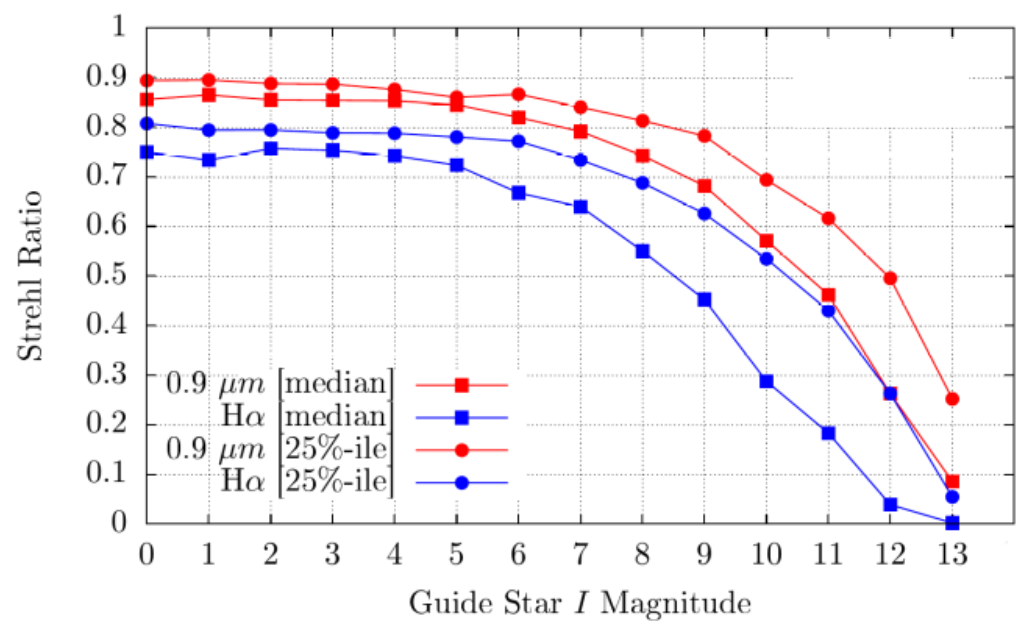
\includegraphics[width=3.1in]{figures/fig1.png}
\vspace{-0.2in}
\caption{ Strehl Ratio vs. guidestar magnitude for 13.5 cm actuator pitch and a 2 kHz ExAO system.  These curves are from MagAO-X simulations \citep{2018SPIE10703E..09M}.  By maintaining the same actuator pitch, these curves can be extrapolated to the GMT ExAO system we propose here. \label{fig:strehl} }
\end{wrapfigure}

The MagAO-X extreme adaptive optics (ExAO) system for the Magellan Clay telescope is currently under construction \citep{2018SPIE10703E..09M, 2018SPIE10703E..4YC}.  It consists of a 2040 actuator deformable mirror (DM), 3.6 kHz pyramid wavefront sensor (PyWFS), a suite of coronagraphs, and employs various post-coronagraph wavefront sensing and control techniques to optimize contrast.  MagAO-X is optimized for work in the visible, red-optical, and near-IR.  Destined for the same site as the GMT, it is an ideal testbed and demonstration system for a potential ExAO system for the GMT.
The concept we describe here, which we call “GMagAO-X” is based on scaling the 2000 actuator DM of MagAO-X from the 6.5 m Clay to the 25.4 m GMT, maintaining the same actuator spacing when projected onto the primary mirror.  This scaling works out to one 3000 actuator DM per 8.4 m diameter segment.  We discuss the opto-mechanical implementation of this below.  Here we note that by preserving projected actuator pitch and AO system speed, such a system will achieve the same Strehl ratio on the GMT as is projected for MagAO-X.  We show this performance in Figure \ref{fig:strehl}.

\begin{wrapfigure}[14]{r}{3.2in}
\centering
\vspace{-0.4in}
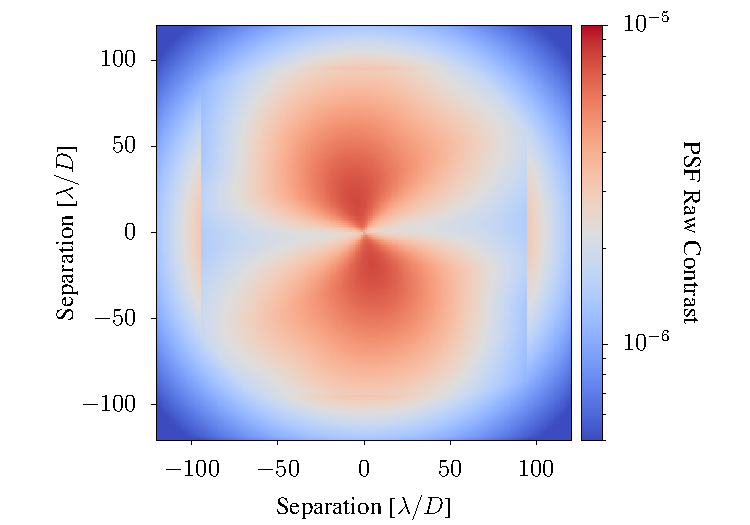
\includegraphics[width=3.1in]{figures/fig2.pdf}
\vspace{-0.2in}
\caption{ Post-coronagraph raw contrast for GMagAO-X using the semi-analytic model of Males and Guyon (2018), for an I=8 mag star such as Prox. Cen.   \label{fig:contrast} }
\end{wrapfigure}

The larger diameter of the GMT results in a significant improvement in post-coronagraph contrast. Due to the finer sampling of atmospheric turbulence power, this improvement goes as $\propto D^2$, hence the GMT will deliver a 15x improvement over the 6.5 m Clay telescope in terms of raw contrast.  The resulting photon-noise limited exposure time improvement goes as $\propto D^4$, and improvement in by a factor of 233.  \citet{2018JATIS...4a9001M} presented a semi-analytic framework for modeling systems such as the one we propose here, including the effects of AO control dynamics.  The result for an I=8th mag star, such as Proxima Centauri, is shown in Figure 2.

\section{Key Science Goals and Objectives}
\textit{The papers should summarize the most important
scientific goals and objectives, justifying the timeliness of the scientific opportunities, and
placing them in as broad a context as possible. We encourage the authors, where relevant, to
reference Science White Papers submitted to the Survey (these are posted on the Astro2020
website, and may be referenced by author and title). Submitters may also make reference to
web sites and other outside materials, but should strive to make this section as self-contained
as possible.}

\subsection{A GMT Survey of Temperate Exoplanets and a Search for Biosignatures on the Nearest Terrestrial Worlds}

To demonstrate the enormous scientific potential of an ExAO+Coronagraph instrument on the GMT, we analyze the existing database of known exoplanets maintained by the NASA Exoplanet Science Institute (NExScI).  For each star with a confirmed exoplanet we normalize any missing parameters, such as luminosity or I magnitude, using a main sequence table.  Most relevant planets are known from radial velocity (RV) surveys.  If no inclination is known, we use $\sin(60)$ to obtain a mass estimate.  The radii of these planets is determined using a mass-to-radius relationship which assumes terrestrial density to $4.1 M_\Earth$ ($1.6 R_\Earth$), and then uses a fit to Neptune, Uranus, Saturn, Jupiter, and the giant planet models of \citet{2007ApJ...659.1661F}.  This relationship is thus well suited to the “lightly irradiated” planets resolvable with the GMT.

Once an exoplanet’s radius is estimated, and its equilibrium temperature estimated from the host star parameters and its orbit, we can estimate its albedo.  For planets $< 1.6 R_\Earth$ we use the Earthshine spectrum of \citet{2006ApJ...644..551T} normalized to EPOXI photometry \citep{2013ApJ...765L..17C}, assuming a Lambertian phase curve. For larger planets, we use the geometric albedo grid of \citet{2010ApJ...724..189C}, which includes phase.  With the radius and geometric albedo, we calculate the mean contrast in reflected light over a planet’s observable orbit.	

Our baseline performance assumptions are that we reach a post-AO contrast of 10x worse than the frozen-flow predictive control predictions of \citet{2018JATIS...4a9001M}.  This is done on a per-guidestar basis, taking into account AO performance as a function of brightness.  The factor of 10 is intended to account for boiling and other non-frozen-flow disturbances, as well as sub-optimal as-built instrument performance. We assume an excellent coronagraph which suppresses the Airy pattern and also suppresses pinning of speckles.   We further assume that post-coronagraph and non-common-path WFS\&C [DEFINE?] is used to suppress quasi-static (long-lived) speckles to a level well below the residual atmospheric speckles.  The resulting residual noise sources are then atmospheric speckles and photon noise.  We include a semi-analytic model of residual atmospheric speckle lifetimes, and thus calculate SNR vs time for an exoplanet of a given brightness with these noise sources.
In Figure \ref{fig:planets} we show the 102 currently-known planets which could be detected in a single night (10 hrs) of telescope time each.  We estimate that a total of roughly 1 month of telescope nights will be needed for the entire survey.  This survey will sample a range of planet radii, including Earth-like and Neptune-like exoplanets.  It also spans a range of equilibrium temperatures corresponding to the inner Solar system.  Planets with these parameters have never been imaged or characterized in reflected light before.

\begin{figure}[h!]
\centering
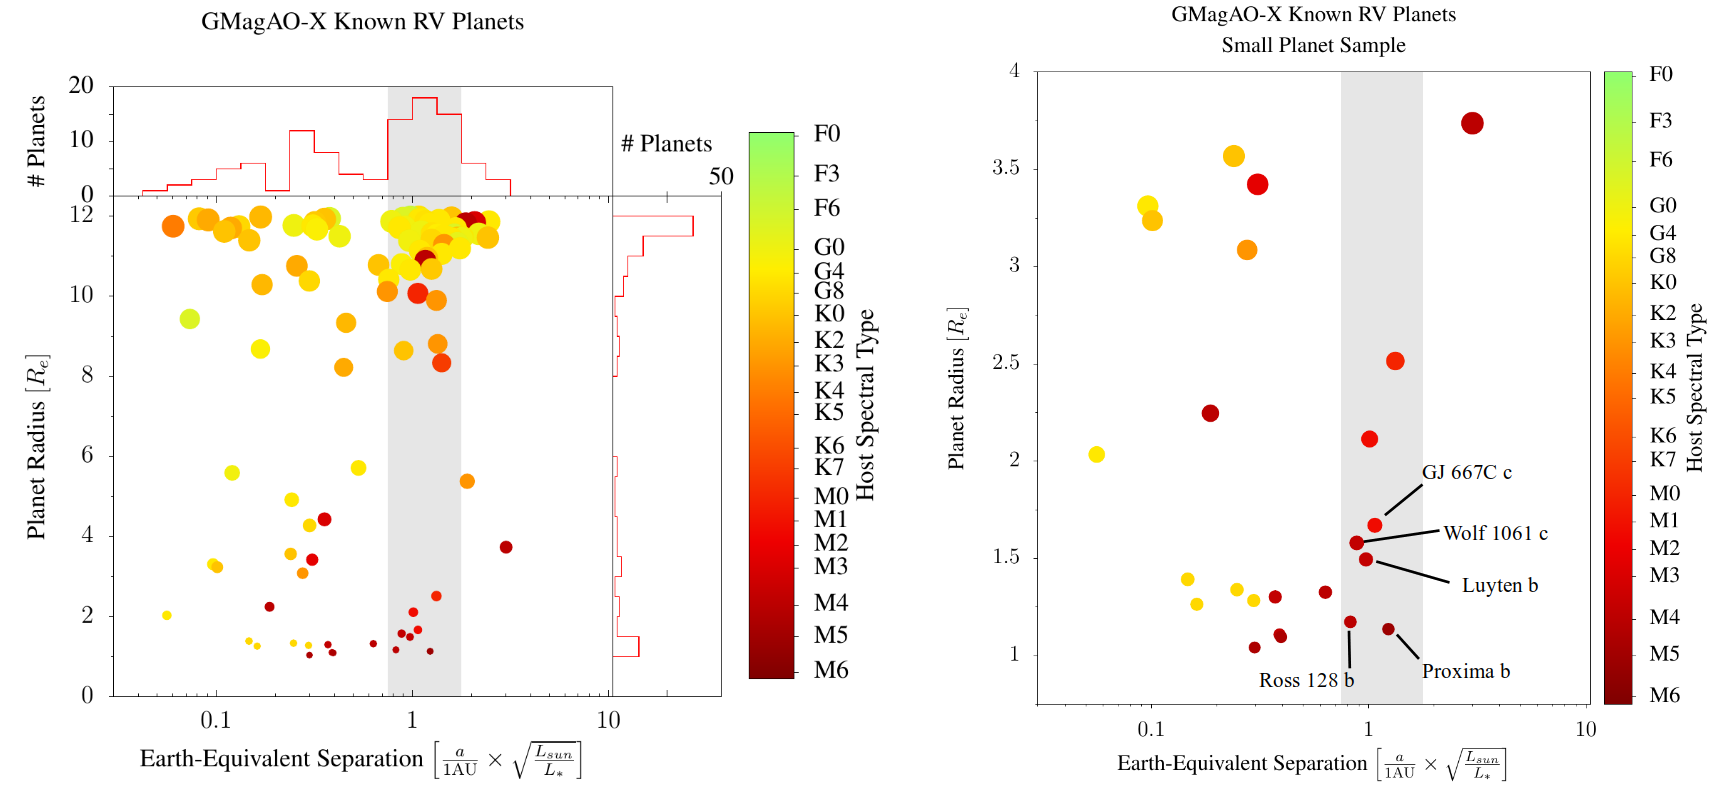
\includegraphics[width=6in]{figures/fig3.png}
\caption{GMagAO-X will enable characterization of over 100 currently known (from RV) planets.  The figure at left shows the full sample, plotted as estimated radius vs. Earth-equivalent separation (or “instellation”).  At right we highlight the small planets, and label the potentially habitable terrestrial planets. \label{fig:planets}}
\end{figure}

In the right hand panel of Figure \ref{fig:planets} we highlight the small ($< R_{Nep}$) sample.  In particular, we note the 5 terrestrial and potentially habitable planets orbiting within the “habitable zone” of their host star.  Once detected in broad-band imaging, these planets will then be characterized in detail.  Characterizing these exoplanets with GMagAO-X in refected light shortly after first-light of the GMT will allow a search for biosignatures around the nearest known temperate terrestrial worlds.
   
Next we assume that we achieve the same level of turbulence rejection, but are only able to suppress quasi-static speckles to a similar level and are hence dominated by long-lived correlated noise.  In this case, we would employ the high dispersion coronagraphy technique \citep[HDC,][]{2017ApJ...838...92M}, where template cross-correlation matching is used to detect the reflected stellar spectrum \citep{2017A&A...599A..16L}.  While less efficient than photometry for short-lived noise sources, HDC allows for root(t) improvement of SNR even in the presence of long-lived spatially correlated speckle noise.  To analyze this case, we use the BT-Settl \citep{2014IAUS..299..271A} to calculate the cross-correlation strength appropriate for a given spectral type, and then estimate the exposure time to detect each exoplanet in the NExScI database. Under this pessimistic performance case, the total number of detected planets (in 10 hrs or less each) is reduced to 63.
In Table 1, we summarize the parameters of the temperate terrestrial (potentially habitable) planets.  Once the initial detection is performed (in the integration times shown), these planets will be extensively characterized to search for biosignatures.

\begin{table}
\caption{Parameters of currently known terrestrial planets to be characterized by GMagAO-X. Here ``detection'' means an initial broad-band albedo measurement.\label{tab:tp}}
\centering
\begin{tabu}{lccccccc}
                &         &             &             &       &    & \multicolumn{2}{c}{ Exp. Time } \\
                &         &             &             &   &        & \multicolumn{2}{c}{ for Detection }  \\
Planet          & Dist.   & Sep.        & Instell.    &  Rad.         & Contrast         & \multicolumn{2}{c}{ [sec] }     \\
                &  [pc]   & [mas]       & $S_{\Earth}$     &  $R_{\Earth}$        &         & Baseline   & Pessimistic \\ 
\hline
\hline
Proxima Cen b    &   1.3  &  37.6  &  1.23  &  1.14  &  1.6$\times 10 ^{-7}$  &  1092 &  2717 \\
Ross128 b       &   3.4  &  14.7   &  0.82  &  1.17  &  1.3$\times 10 ^{-7}$  &  4674  &  9388 \\
Luyten b         &   3.8   &  24.0   &  0.97  &  1.49  &  8.1$\times 10 ^{-8}$  &  3859  &  6092 \\
Wolf 1061 c     &   4.3  &  20.6   &  0.88  &  1.58  &  9.3$\times 10 ^{-8}$  &  2844  &  5650 \\
GJ 667C c        &  6.8   &  18.4   &  1.0  &  1.66  &  8.2$\times 10 ^{-8}$  &  14849  &  36157 \\
\hline
\end{tabu}
\end{table}

REFERENCE SCIENCE WHITE PAPERS

\subsection{ H-alpha Planets}
LAIRD PLEASE ADD.  

REFERENCE SCIENCE WHITE PAPERS

\subsection{ Other Exoplanet Science}

REFERENCE SCIENCE WHITE PAPERS

\subsection{ Disks }

REFERENCE SCIENCE WHITE PAPERS

\subsection{ Stellar Spectra}

REFERENCE SCIENCE WHITE PAPERS

\section{Technical Overview}
\textit{The team should provide a description of the technical aspects of the
pursuit, including a description of the essential performance parameters for achieving the
project's science goals.}
\textit{For ground-based activities/projects, papers should describe the telescope or
observatory architecture, key performance requirements, technical requirements,
anticipated site and infrastructure requirements, as well as any public/private
partnerships.}

TECHNICAL DESCRIPTION OF GMT (including site, consortium, etc)

In Figure \ref{fig:ap} we present our notional concept of how the GMagAO-X instrument could be mounted in a gravity invariant environment at the so-called Auxilliary Port (AP). The AP is essentially equivalent to a Nasmyth port on the GMT, being on the elevation axis and so is the only place on GMT that is both gravity invariant and can also be used for imaging.  Figure 4 shows how GMagAO-X will appear when mounted at the elevation axis on the GMT. As the telescope moves in elevation the instrument stays fixed w.r.t. gravity. A floating optical table (with servo control on the position of the table-- utilizing the TMC PEPSII stability system) can be employed.  This will prevent vibrations above 10Hz from coupling into the instrument (lower frequency vibrations will be removed by the AO system). 
This notional concept has established the feasibility of mounting GMagAO-X on the GMT without conflicts with already planned instruments.  The next step is to perform a conceptual design study to ensure that such an instrument will achieve the demanding science based requirement we motivate above, and addresses the risks unique to this instrument. 

\begin{figure}
\centering
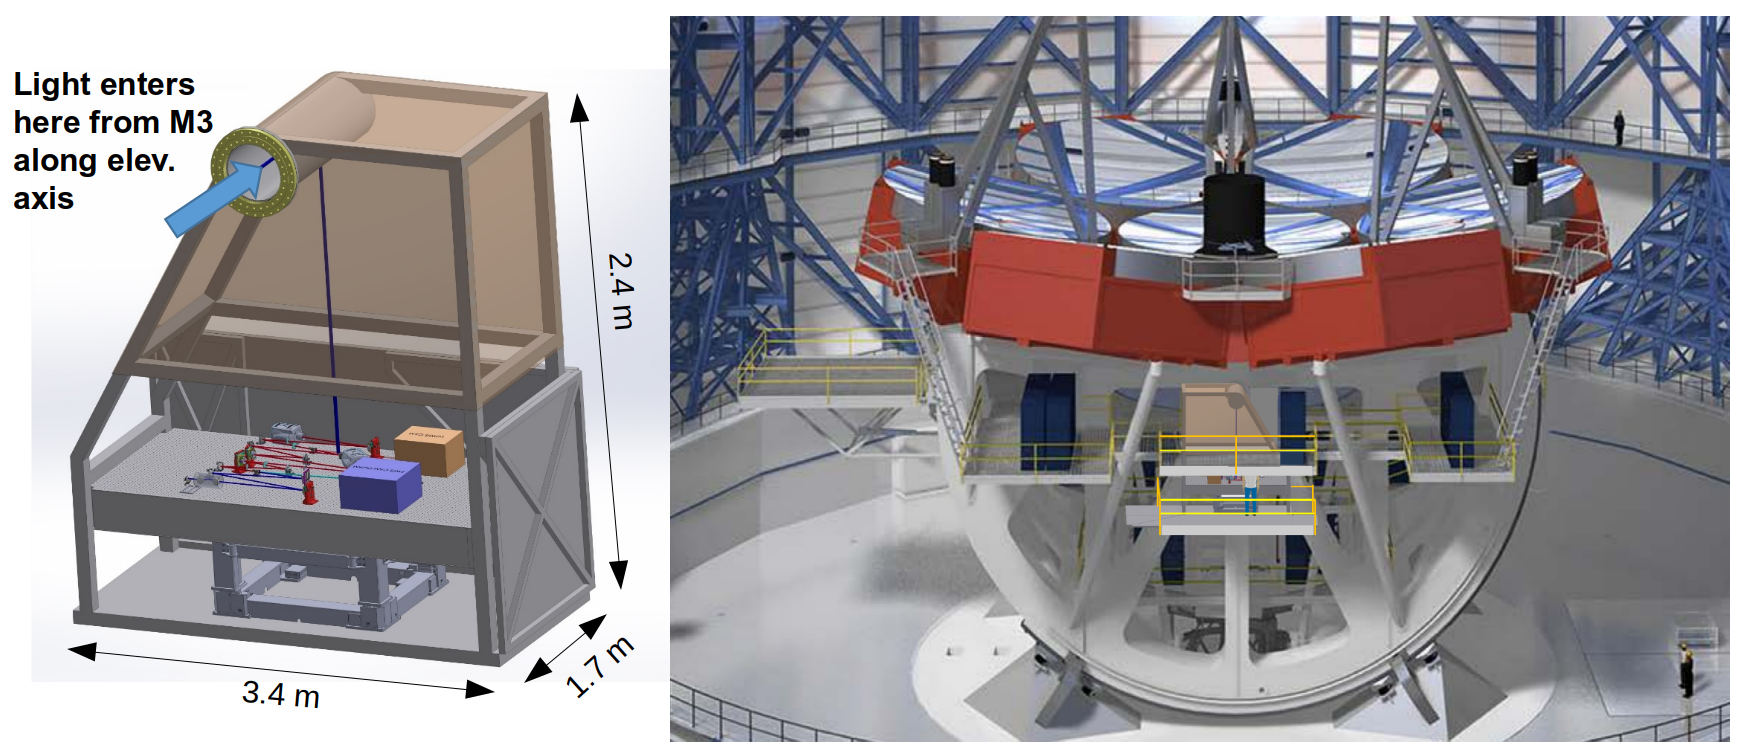
\includegraphics[width=6in]{figures/ap.png}
\caption{ GMagAO-X concept shown within the Aux. Port volume and mounted on the GMT elevation axis. \label{fig:ap}}
\end{figure}

\section{Technology Drivers} 
\textit{If the pursuit requires new technologies, the paper should identify and
describe them, along with an outline of technology maturation plans and timescales.}

PUT PHASING TESTBED STUFF HERE

\section{Organization, Partnerships, and Current Status}  
\textit{All pursuits should describe the participating
organizations, any planned partnerships, and their current status.}

\section{Schedule}
\textit{The team should outline the development and operations schedule. The schedule
should also indicate the operational lifetime of the pursuit.}

\section{Cost Estimates}
\textit{The team should provide any cost estimates that have been developed for the
current version of the pursuit. This should include the date the cost estimate was performed,
should reference the base fiscal year, the organization that performed the estimate, and the top
level results of the estimate, broken out by the major development and operational phases.
Operating costs should be divided into direct funding to the science community (if planned) and
costs required to keep facilities, missions, or other necessary infrastructure running. Any
unusual end-of-life (e.g. decomissioning) costs should be noted. Also, if applicable, a
breakdown of the assumed funding from federal, other public, international, or private sources
should be provided. Specific sources of funding need not be identified.
MODIFICATION: The team should provide completed cost estimates if available. If costs are
still being developed and validated, or the breakdown of funding is yet to be determined, the
project should provide the cost category for the overall project, including science and
operations. The categories are:}

Ground
-------------


Small $<$\$20M

Medium \$20M - 70M

Large $>$\$70M


\clearpage
\thispagestyle{empty}
% References
\bibliography{references} % bibliography data in report.bib
\bibliographystyle{apj} % makes bibtex use spiebib.bst

\end{document}

% End of file `sample62.tex'.
